\subsubsection{Neuronal Plasticity in the Adult Brain}
\index{Zupanc, G�nther K.H. }

\paragraph{Research Team}
G�nther K.H. Zupanc (Professor), Marianne M. Zupanc (Postdoctoral Research Associate), Karen Hinsch (Graduate Student/Postdoctoral Fellow), R. Samuel Rajendran (Graduate Student), Ursula M. Wellbrock (Lab Technician), Jos� Antonio Gama Salgado (Lab Technician)\\


Contrary to a long-held dogma, the vertebrate brain continues to generate new neurons throughout adulthood. However, while in mammals (including humans) this so-called adult neurogenesis is restricted to just two brain regions, and the number of new neurons is extremely low, in bony fish numerous new neurons are continuously produced in many regions of the adult brain. As a consequence and in contrast to mammals, fish exhibit an enormous potential for structural and functional brain repair after injuries. Capitalizing on this advantage, the research of my laboratory aims to explore cellular mechanisms, behavioral consequences, and the evolutionary development of neurogenesis in the adult fish brain. Towards this goal, we employ an integrative approach, combining neuroanatomical, neurophysiological, neuropharmacological, molecular, and behavioral techniques. This research has not only answered fundamental biological questions, but could also provide the foundation to define novel therapeutic strategies to replace neurons lost to injury or neurodegenerative disease by newly generated ones.

\begin{figure}[ht]
  \begin{center}
   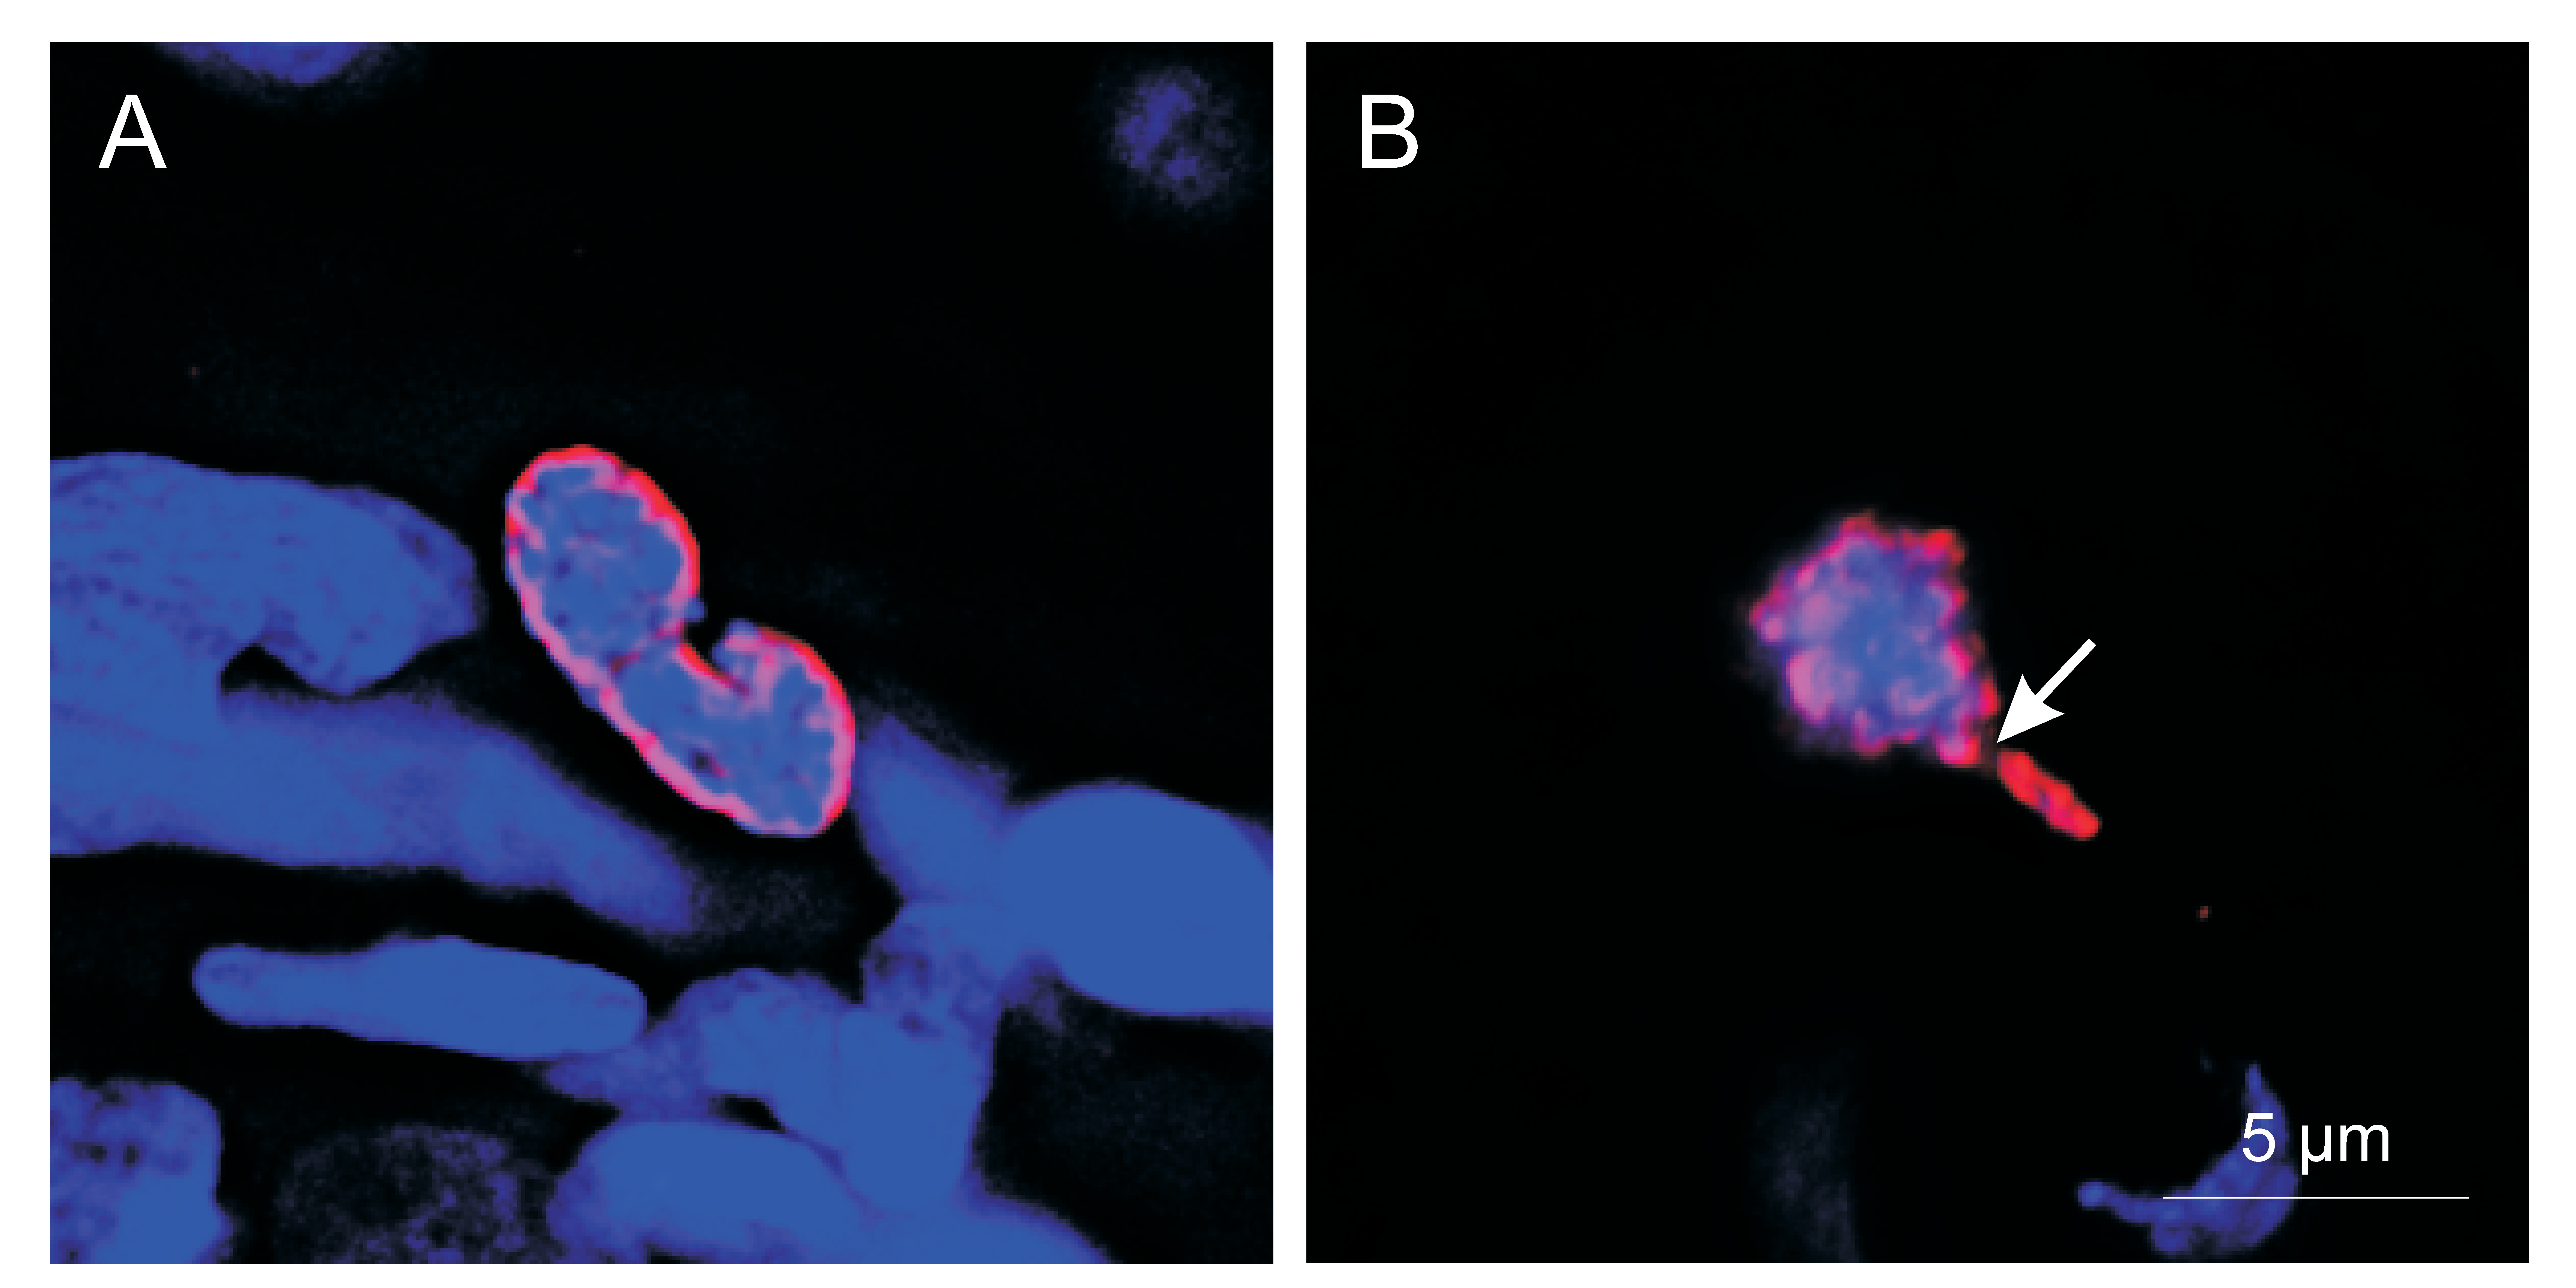
\includegraphics[width=\hsize]{Zupanc/Zupanc_fig.pdf}
    \mycaption{ High-power images of mitotically dividing cell nuclei in the adult fish brain. \textbf{A}: Normal mitotic profile. The cell divides symmetrically, resulting in two equally large daughter nuclei. \textbf{B}: Asymmetric division. The cell divides into one larger daughter nucleus and another rather small piece of nuclear material, a so-called laggard. These two chromosomal portions are separated by a clear gap (arrow). As a result, one of these daughter nuclei contains more chromosomes, whereas the other has less chromosomes, than the normal, euploid set of chromosomes found in each daughter nucleus after symmetric division. Modification of chromosome number is a novel mechanism that regulates gene activity during development. (Modified after Rajendran et al., in press.)}\label{fig:Zupanc}
   \end{center}
\end{figure}

\paragraph{Highlights}\noindent

(1) By employing differential proteome analysis, we have performed the first large-scale identification of proteins involved in tissue repair in the adult vertebrate brain (Zupanc et al., 2006). The results of this investigation suggest several hundreds of proteins to be associated with neuronal regeneration. Twenty-four of these proteins were identified by peptide mass fingerprinting and mass spectrometry/mass spectrometry fragmentation. Among them are a number of novel proteins that have never before been reported to be involved in brain regeneration. Since the mechanisms that control neuronal development and regeneration are very similar among vertebrates, the results obtained through this study have provided new insights into the factors that limit brain repair in mammals, including humans.

(2) One of the cellular factors that is involved in regeneration of the adult fish brain after injuries is the calcium-binding protein calbindin-$\mbox{D}_{\mbox{{\footnotesize 28k}}}$. By combining a cerebellar lesion paradigm developed in our laboratory with immunohistochemical staining and analysis by both fluorescence microscopy and confocal microscopy, we characterized the spatiotemporal expression pattern of this protein after brain injury (Zupanc and Zupanc, 2006). Our results suggest that calbindin-$\mbox{D}_{\mbox{{\footnotesize 28k}}}$ exerts a neuroprotective function by buffering free intracellular calcium ions, whose concentration is elevated after brain insults.

(3) As the first research group worldwide, we have succeeded in the isolation and purification of stem cells from the adult fish brain (Hinsch and Zupanc, 2006). These cells exhibit the ability for self-renewal and, under proper conditions, gave rise to both neurons and glia cells. The possibility to maintain and propagate these cells in vitro provides now excellent opportunities to characterize the cellular factors that mediate the proliferation and differentiation of the new cells in the adult fish brain.

(4) In contrast to the traditional view that developmental regulation of cell proliferation and differentiation operates on a constant genome and is restricted to alterations at transcriptional and posttranslational levels, we could provided evidence for somatic genomic alterations, resulting in a genetic mosaic of the new cells in the adult fish brain (Rajendran et al., in press).  This genomic alteration is manifested as aneuploidy (chromosome number different from the normal, euploid specifies-specific set of chromosomes) and appear to form the basis for a novel mechanism to regulate gene expression during development.

(5) As part of our effort to establish a behavioral paradigm to study the functional consequences of adult neurogenesis, we have performed a comprehensive ethological and biophysical analysis of chirping behavior (Zupanc et al., 2006). This electric behavioral pattern, produced by certain weakly electric fish, is controlled by a well-characterized brain nucleus in the diencephalon. As previous studies from our laboratory have shown, the underlying neural network undergoes pronounced structural reorganization caused by the generation of new neurons. These structural alterations correlate with dramatic behavioral changes. Our recent study has shown that chirping is composed of different chirp types that are distinct in terms of their biophysical properties. We, furthermore, succeeded as the first group worldwide to perform simultaneous recordings from electrically interacting fish, which provided the basis for the demonstration of an important communicatory function of the chirping behavior.




%\paragraph{Activities}
%\begin{enumerate}
%\item Research visits: Laboratory of Genetics, The Salk Institute for Biological Studies and Section of Neurobiology, Division of Biological Sciences, University of California, San Diego; both in La Jolla, California, USA; June-August 2006
%\item Invited Lectures: Link�ping University (Sweden); University of Vienna and Austrian Neuroscience Association (Austria); University of California, San Diego (USA); University of Sheffield (UK)
%\item Vertrauensdozent, Friedrich Ebert Foundation, Bonn, Germany
%\item Advisory Board, International School of Bremen, Germany
%\end{enumerate}

\paragraph{Organization}
\begin{enumerate}
\item Appointment to the Editorial Advisory Board of
``Journal of Comparative Physiology A'', Springer-Verlag, Berlin/Heidelberg (2006)

\item Appointment to Senior Editor of  ``Journal of Zoology'', Blackwell Publishing, Oxford/Edinburgh, published on behalf of the Zoological Society of London (2007)
\end{enumerate}


\myparagraph{Collaborations}
%
Bremen Area Collaborations:
\begin{enumerate}
\item {\sl International University Bremen} \\ Prof. C.C. Hilgetag \\ Modeling of development of neural networks
\end{enumerate}
National \& International Collaborations:
\begin{enumerate}
\item {\sl The Scripps Research Institute, La Jolla, California, USA }\\ Prof. J. Chun \\ Chromosomal analysis of neuronal stem cells derived from the adult brain
\item {\sl Salk Institute for Biological Studies, La Jolla, California, USA} \\ Prof. F.H. Gage \\ Adult neurogenesis in the vertebrate brain
\item {\sl Interdisciplinary Center of Clinical Research Leipzig, University of Leipzig, Leipzig, Germany} \\ Dr. A. L�sche \\ Chromosomal analysis of neuronal stem cells derived from the adult brain
\end{enumerate}


\paragraph{Grants}
\begin{enumerate}
\item Funded by Wilhelm Herbst Stiftung,  \emph{Molecular
Identification of Permissive Factors Associated with Neuronal
Regeneration}, (Sepember 2005 - February 2006)
 \item Funded by T�njes Vagt Stiftung,  \emph{Replacement of Injured Brain Cells by Newly Generated
Neurons}, (February 2006 - December 2007)
\end{enumerate}

\nocite{Zupanc1,Zupanc2,Zupanc3,Zupanc4,Zupanc5,Zupanc6,Zupanc7,Zupanc8,Zupanc9,Zupanc10,Zupanc11,Zupanc12,Zupanc13,Zupanc14}
